\subsection{Results for Heading}
%\label{subsec:direction_results}
%\vspace{10pt}

Figure~\ref{fig:var_direction} represents the $p$-values for the Wilcoxon signed-rank test on actual and predicted values across $k$-fold validation datasets for the heading in the $k$-fold testing datasets using different RNN models, and forecasting times. Darker colors in grayscale represent a higher $p$-value in a range from $0$ to $1$. The values on the secondary diagonal are all equal to $1$ and black because models equal themselves.

\begin{figure}[!ht]
	\centering
	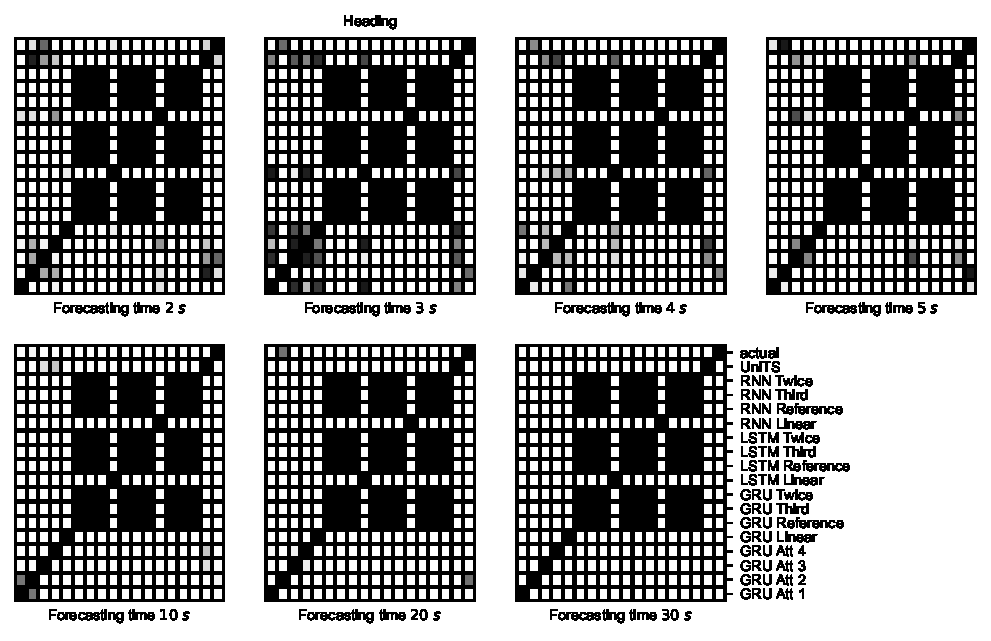
\includegraphics[width = 0.99 \linewidth]{var_direction.pdf}
	\caption{The $p$-values for the Wilcoxon signed-rank test on actual and predicted values across $k$-fold validation datasets for the heading in the $k$-fold testing datasets using different RNN models, and forecasting times. Darker colors in grayscale represent a higher $p$-value in a range from $0$ to $1$. The values on the secondary diagonal are all equal to $1$ and black because models equal themselves.}
	\label{fig:var_direction}
\end{figure}

Figure~\ref{fig:best_RMSE_val} contains the average RMSE across $k$-fold testing datasets using different validation datasets for all variables estimated in nested $k$-fold cross-validation by different RNN models, and forecasting times.

\begin{figure}[!ht]
	\centering
	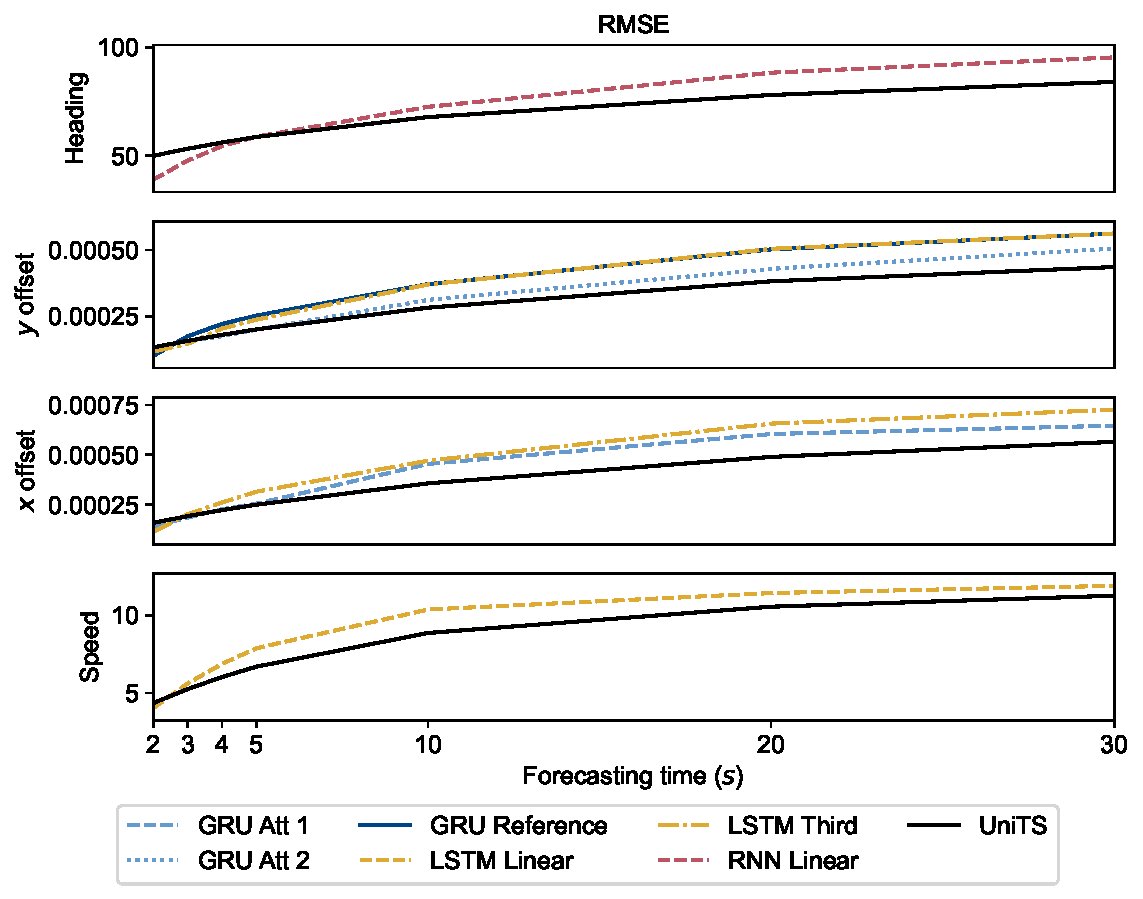
\includegraphics[width = 0.99 \linewidth]{best_RMSE_val.pdf}
	\caption{The average RMSE across $k$-fold testing datasets using different validation datasets for all variables estimated in nested $k$-fold cross-validation by different RNN models, and forecasting times.}
	\label{fig:best_RMSE_val}
\end{figure}

The average RMSE, with standard deviation in brackets, across $k$-fold validation datasets for the heading estimated on the $k$-fold testing datasets by different RNN models, and forecasting times is listed in Table~\ref{tab:best_direction_RMSE}.

\begin{table}[!ht]
	\centering
	\resizebox{\linewidth}{!}{
		\begin{tabular}{|c|c|c|c|c|c|c|c|}
			\hline
			Model & $2$ $s$ & $3$ $s$ & $4$ $s$ & $5$ $s$ & $10$ $s$ & $20$ $s$ & $30$ $s$ \\ \hline
			\multirow{2}{*}{RNN Linear} & $\mathbf{38.85}$ & $\mathbf{47.63}$ & $\mathbf{54.36}$ & $58.71$ & $72.54$ & $88.35$ & $95.47$ \\
			 & \textbf{(}$\mathbf{1.85}$\textbf{)} & \textbf{(}$\mathbf{2.42}$\textbf{)} & \textbf{(}$\mathbf{2.22}$\textbf{)} & ($2.05$) & ($2.33$) & ($1.93$) & ($2.48$) \\ \hline
			\multirow{2}{*}{UniTS} & $49.88$ & $53.14$ & $56.02$ & $\mathbf{58.6}$ & $\mathbf{67.8}$ & $\mathbf{78.04}$ & $\mathbf{84.09}$ \\
			 & ($2.18$) & ($2.29$) & ($2.35$) & \textbf{(}$\mathbf{2.38}$\textbf{)} & \textbf{(}$\mathbf{2.26}$\textbf{)} & \textbf{(}$\mathbf{2.29}$\textbf{)} & \textbf{(}$\mathbf{2.47}$\textbf{)} \\ \hline
		\end{tabular}
	}
	\caption{The average RMSE, with standard deviation in brackets, across $k$-fold validation datasets for the heading estimated on the $k$-fold testing datasets by different RNN models, and forecasting times.}
	\label{tab:best_direction_RMSE}
\end{table}

The RNN Linear model achieved the lowest RMSE for heading, and a forecasting time of $2$, $3$, and $4$ $s$ with average values and standard deviation (in brackets) that equal $38.85$ $\degree$ ($1.85$ $\degree$), $47.63$ $\degree$ ($2.42$ $\degree$), and $54.36$ $\degree$ ($2.22$ $\degree$) respectively.

The RNN Linear model does not have a statistically significantly different RMSE than the GRU Linear model for heading using a forecasting time of $2$ $s$, with a $p$-value equaling $3.764 \times 10^{-4}$.

\markertable{tab:\label{tab:RMSE:direction:p:2}}

The RNN Linear model does not have a statistically significantly different RMSE than the GRU Linear, and LSTM Linear models for heading using a forecasting time of $4$ $s$, with $p$-values equaling $5.564 \times 10^{-4}$, and $4.895 \times 10^{-4}$.

\markertable{tab:\label{tab:RMSE:direction:p:4}}

The UniTS model achieved the lowest RMSE for heading, and a forecasting time of $5$, $10$, $20$, and $30$ $s$ with average values and standard deviation (in brackets) that equal $58.6$ $\degree$ ($2.38$ $\degree$), $67.8$ $\degree$ ($2.26$ $\degree$), $78.04$ $\degree$ ($2.29$ $\degree$), and $84.09$ $\degree$ ($2.47$ $\degree$) respectively.

The UniTS model does not have a statistically significantly different RMSE than the LSTM Linear, and RNN Linear models for heading using a forecasting time of $5$ $s$, with $p$-values equaling $2.785 \times 10^{-3}$, and $6.721 \times 10^{-1}$.

\markertable{tab:\label{tab:RMSE:direction:p:5}}

